\section{Methodology}
\label{sec:methods}

Fig.~\ref{fig:workflow} shows the inputs, the model and the three evaluation settings. The fleet oracle and the MOS branch are diagnostic arms and are never part of a deployed configuration.

\begin{figure}[!htb]
\centering
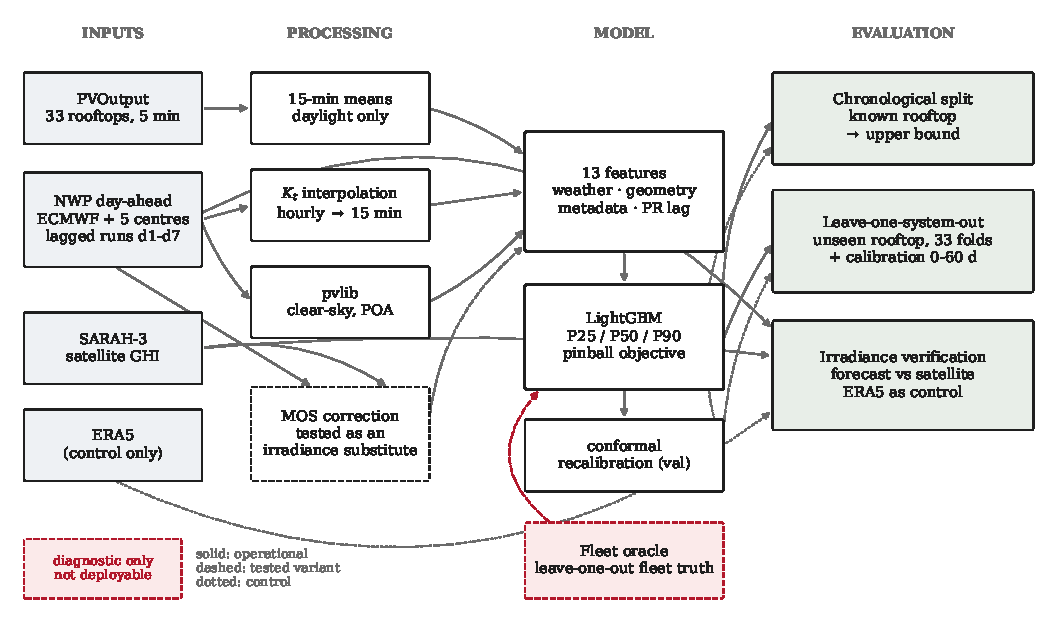
\includegraphics[width=\textwidth]{figures/fig3_workflow.pdf}
\caption{Methodology. Solid paths are operational: every input exists at the noon issue time of the preceding day. The dashed MOS branch supplies corrected irradiance as a substitute input. The shaded fleet oracle uses information unavailable at forecast time. ERA5 enters only as a control reference.}
\label{fig:workflow}
\end{figure}

\subsection{Forecast task and baseline}
\label{sec:meth-task}

For each system and each 15-min daylight slot of the following day, the model predicts output normalised by rated capacity,
\begin{equation}
y = P / (1000\,C_\mathrm{p}),
\end{equation}
with $P$ the AC output in W and $C_\mathrm{p}$ the rated DC capacity in kW$_\mathrm{p}$, clipped to $[0, 1.2]$ because real systems briefly exceed nameplate in cold, bright conditions. Normalisation lets systems of different size be learned jointly. The forecast is issued around noon of the preceding day and uses only information available then. The reference forecast is persistence, the same slot one day earlier, and skill is
\begin{equation}
S = 1 - \mathrm{RMSE}_\mathrm{model} / \mathrm{RMSE}_\mathrm{persistence}.
\end{equation}
Skill is the headline metric (Section~\ref{sec:rw-prob}). Because part of the previous day is not yet observed at noon, this persistence is slightly optimistic, so the reported skill is conservative.

\subsection{Features}
\label{sec:meth-features}

Thirteen features enter the final model (Table~\ref{tab:features}). Plane-of-array irradiance uses the Hay--Davies transposition \citep{Hay1979} in pvlib \citep{Holmgren2018} with the reported tilt and azimuth. The only site-specific history is a lagged performance ratio,
\begin{equation}
pr = y \,/\, \max(\mathrm{GHI}_\mathrm{cs}/1000,\; 0.05),
\end{equation}
taken at the same slot two days earlier, because the previous day is incomplete at noon. Lagging the ratio rather than raw output carries persistent site properties such as shading, soiling and derating, without letting yesterday's weather bias tomorrow's forecast. All NWP features are issued before the noon cutoff, so no feature uses information unavailable at issue time.

\begin{table}[!htb]
\centering
\caption{The thirteen model features. Source: E, ECMWF IFS day-ahead; I, DWD ICON day-ahead; M, mean of six centres; G, solar geometry; R, owner-reported record; H, the rooftop's own history.}
\label{tab:features}
\small
\begin{tabularx}{\textwidth}{@{}r X l l@{}}
\toprule
\# & Feature & Unit & Src \\
\midrule
1 & Plane-of-array irradiance (ECMWF) & W\,m$^{-2}$ & E \\
2 & Plane-of-array irradiance (ICON) & W\,m$^{-2}$ & I \\
3 & Clear-sky GHI, Ineichen--Perez & W\,m$^{-2}$ & G \\
4 & Direct normal irradiance & W\,m$^{-2}$ & E \\
5 & Total cloud cover & \% & I \\
6 & Multi-model mean GHI (ECMWF, ICON, GFS, M\'et\'eo-France, DMI, UK Met Office) & W\,m$^{-2}$ & M \\
7 & Solar elevation & $^\circ$ & G \\
8 & Solar azimuth & $^\circ$ & G \\
9 & $\cos(2\pi \cdot \text{minute of day} / 1440)$ & -- & G \\
10 & Rated DC capacity & kW$_\mathrm{p}$ & R \\
11 & Array tilt & $^\circ$ & R \\
12 & Array azimuth & $^\circ$ & R \\
13 & Performance ratio, same slot two days earlier & -- & H \\
\bottomrule
\end{tabularx}
\end{table}

\subsection{Model and hyperparameter selection}
\label{sec:meth-model}

Forecasts come from LightGBM gradient-boosted trees \citep{Ke2017,Friedman2001}. One model is fitted for each quantile $\alpha \in \{0.25, 0.50, 0.90\}$, each minimising the pinball loss
\begin{equation}
L_\alpha(y, \hat{y}) = \max\left[\alpha (y - \hat{y}),\; (\alpha - 1)(y - \hat{y})\right],
\end{equation}
whose minimiser is the conditional $\alpha$-quantile \citep{Koenker1978}. P50 serves as the point forecast. Predictions are clipped to $[0, 1.2]$.

Two hyperparameter searches use a tree-structured Parzen estimator in Optuna \citep{Akiba2019}, each for a different population.

\textbf{Temporal search (known rooftops).} Sixty trials per quantile minimise the pinball loss at that quantile on the validation split. Within the training split, the first 85\% fits the trees and the last 15\% sets early stopping, so the stopping rule and the selection never share data. The comparison is a preliminary configuration selected by 20 trials minimising validation RMSE under squared error and reused for all quantiles (experiment E0).

\textbf{Transfer search (unseen rooftops).} The inner loop holds out whole systems instead of future dates. The systems of a 45\% row subsample of the training and validation periods are split into three folds of eleven. Each trial trains on two folds and is scored by P50 pinball loss on the held-out systems, with early stopping on a time-tail of the training systems. Forty trials were run for P50 only.

The temporal configuration is used for every experiment on the chronological split; the transfer configuration is used for P50 in every leave-one-system-out experiment. The two are never compared as interchangeable.

\subsection{Ensemble constructions}
\label{sec:meth-ens}

Three ways of widening the weather input are compared, all at a day-ahead lead time. A \emph{lagged ensemble} averages ECMWF runs issued one to seven days before the target. A \emph{multi-model ensemble} averages the day-ahead GHI of the six centres, ignoring missing members (feature 6). \emph{Ensemble dispersion} supplies the standard deviation across all twelve members, across lagged members and across centres, the interquartile range and the fraction of members within $\pm 15\%$ of the mean.

\subsection{Fleet oracle}
\label{sec:meth-oracle}

To bound the value of perfect regional weather knowledge, the oracle feature for system $i$ at time $t$ is the mean measured output of all other systems at the same instant,
\begin{equation}
o(i, t) = \frac{\sum_j y(j, t) - y(i, t)}{n(t) - 1},
\end{equation}
with $n(t)$ the number of systems reporting, and used only where $n(t) > 3$. Thirty-three rooftops across Belgium form a distributed irradiance sensor network, so $o(i,t)$ is a close proxy for what the regional sky did. Three arms are compared on identical rows: the baseline features, the baseline plus the oracle, and the oracle with solar geometry and metadata but no NWP.

\subsection{Verification and recalibration}
\label{sec:meth-verif}

Point accuracy is reported as MAE, RMSE, mean bias error (MBE, observed minus predicted, so positive means under-forecasting), $R^2$ and skill. Irradiance bias is reported as forecast minus reference, so positive means over-forecasting, following \citet{Tuononen2019}. Probabilistic quality is reported as the mean pinball loss over the three quantiles, a proper score \citep{Gneiting2007}, as reliability, the empirical frequency of observations below each quantile \citep{Lauret2019}, and as coverage of the P25--P90 band against its nominal 0.65. Errors are stratified by the \emph{forecast} clear-sky index, which is known when decisions are made. Stratifying by the observed index conditions on the target and makes $R^2$ uninterpretable within bins, so only RMSE and bias are read from that view.

Raw quantile regression under-covers at the tails. A conformal-style offset \citep{Romano2019} is fitted on the validation split and applied unchanged to the test split,
\begin{equation}
\delta_q = \mathrm{Quantile}_q\!\left(y_\mathrm{val} - \hat{y}_{\mathrm{val},q}\right), \qquad \hat{y}_{\mathrm{test},q} \leftarrow \mathrm{clip}\!\left(\hat{y}_{\mathrm{test},q} + \delta_q,\; 0,\; 1.2\right).
\end{equation}

\subsection{Model output statistics}
\label{sec:meth-mos}

MOS is tested in two stages. At the \emph{irradiance stage}, a model learns the forecast error, truth minus ECMWF GHI, from ten predictors available at issue time: ECMWF GHI, cloud cover and temperature, clear-sky GHI, the forecast clear-sky index, solar elevation, and sine--cosine pairs of time of day and day of year. Ridge regression, random forest, LightGBM and XGBoost are compared. Two arms differ only in the truth: SARAH-3 or ERA5.

At the \emph{power stage}, the corrected irradiance enters the PV model. Because the correction becomes an input, it is produced out of fold: training rows are corrected by models fitted on the other four of five chronological folds, and validation and test rows by a model fitted on the full training split. The correction is applied to the 15-min GHI and plane-of-array irradiance as a ratio, which preserves night-time zeros and the daily shape.

\subsection{Leave-one-system-out and local calibration}
\label{sec:meth-loso}

Each system is held out in turn. A model trained on the other 32 systems over the training and validation periods predicts the held-out system's test window, giving 33 zero-shot results. The first $N \in \{3, 7, 14, 30, 45, 60\}$ days of that window then fit a local correction, and the rest is scored. Four corrections are compared: none; a \emph{bias} offset equal to the mean residual; \emph{linear} rescaling, $y \approx a + b\hat{y}$; and \emph{capacity + bias}, which first rescales by the observed capacity relative to the fleet,
\begin{equation}
s = \frac{P_{99,\mathrm{cal}} / C_\mathrm{p}}{\mathrm{median}_\mathrm{fleet}\left(P_{99} / C_\mathrm{p}\right)}, \qquad s \in [0.4, 2.5],
\end{equation}
with the fleet median taken from training systems only, and then removes the residual offset. The evaluation window shrinks and moves later in the season as $N$ grows, so corrections are compared only at equal $N$.

\subsection{Experiments}
\label{sec:meth-exp}

Table~\ref{tab:experiments} lists the experiments. Each varies one factor and holds the rest fixed. All numbers in Section~\ref{sec:results} were produced by a single driver with the quantile objective, the final feature build, the splits of Section~\ref{sec:data-splits} and SARAH-3 for irradiance scoring. Computations used Python 3.12, LightGBM 4.6.0, scikit-learn 1.9.0, pandas 3.0.3 and pvlib on a 12-core workstation. The Supplementary material gives the selected hyperparameters, full result tables and computation details.

\begin{table}[!htb]
\centering
\caption{Experiments. Split: T, chronological; L, leave-one-system-out.}
\label{tab:experiments}
\small
\begin{tabularx}{\textwidth}{@{}l >{\raggedright\arraybackslash}X >{\raggedright\arraybackslash}X l@{}}
\toprule
ID & Question & Varied & Split \\
\midrule
E0 & Does the selection objective matter? & RMSE vs pinball selection & T \\
E1 & What is perfect regional weather worth? & oracle; NWP present or absent & T \\
E2 & Where does the residual error live? & stratification only & T \\
E3 & Which input widening helps? & feature subset (7 arms) & T \\
E4 & What is the proposed configuration worth? & ensemble feature; system 81376; recalibration & T \\
E5 & What does an unseen rooftop receive? & held-out system; calibration window and method & L \\
MOS & Does irradiance correction reach power? & raw or corrected irradiance & T, L \\
\bottomrule
\end{tabularx}
\end{table}
